\question{9.5}{
    Een broodjeszaak langs een drukke provinciale weg heeft al een aantal jaren bijgehouden hoeveel klanten er komen tijdens de lunchperiode.
    Dat leverde een tamelijk stabiel patroon op met een gemiddelde van $\mu=42$ klanten per dag en een standaarddeviatie $\sigma=5$.
    Twee maanden geleden is er bij een dichtbij gelegen benzinestation een voorziening gekomen waar klanten snacks kunnen verkrijgen.
    De eigenaar van de broodjeszaak maakt zich zorgen en heeft gedurende $50$ dagen het aantal klanten geteld dat bij hem komt tijdens de lunchperiode.
    Dat leverde een gemiddelde op van $37,8$ klanten.
    Toets eenzijdig of hier sprake is van een significante daling ($\alpha=0,05$).
}
\answer{
    In deze hypothesetoets geldt dat de nulhypothese $H_0: \mu \ge 42$ (geen daling) getest wordt tegen de alternatieve hypothese $H_1: \mu < 42$ (wel een daling).
    
    Omdat we linkszijdig toetsen, berekenen we de $z$-waarde
    \[
        z_{\alpha} = \invnorm(opp=1-\alpha) = \invnorm(opp=0,95) \approx 1,6449
    \]

    De toetsingsgrootheid is in dit geval het (theoretische) steekproefgemiddelde $\overline{X}$.
    Uit de centrale limietstelling volgt dat $\overline{X} \sim N(\mu; \frac{\sigma}{\sqrt{n}})$.
    Onder de aanname dat $H_0$ waar is, geldt dat het gemiddelde $\mu = 42$.
    Verder geldt dat de standaardafwijking $\sigma = 5$ bekend is en de eigenaar $50$ waarnemingen doet, oftewel $n=50$.
    Er volgt dus dat $\sigma(\overline{X}) = \frac{\sigma}{\sqrt{n}} = \frac{5}{\sqrt{50}}$, oftewel $\overline{X} \sim N(\mu=50; \sigma=\frac{5}{\sqrt{50}})$.
    Merk op dat hoe lager het steekproefgemiddelde is, hoe waarschijnlijker dat de alternatieve hypothese waar is.
    Het kritieke gebied is dus van de vorm $(-\infty, g]$, waarbij $g$ kan worden berekend als volgt:
    \begin{align*}
        g   &= \mu - z_{\alpha} \cdot \frac{\sigma}{\sqrt{n}} \\
            &= 42 - 1,6449 \cdot \frac{5}{\sqrt{50}} \\
            &\approx 40,8369
    \end{align*}

    Het kritieke gebied is dus gelijk aan $(-\infty; 40,8369)$.
    Het geobserveerde steekproefgemiddelde $\overline{x}=37,8$ ligt in het kritieke gebied, dus we verwerpen $H_0$.
    Er is voldoende reden om aan te nemen dat het gemiddelde aantal klanten per dag in de broodjeszaak significant is gedaald. 

    \begin{center}
        \resizebox{0.9\textwidth}{!}{
            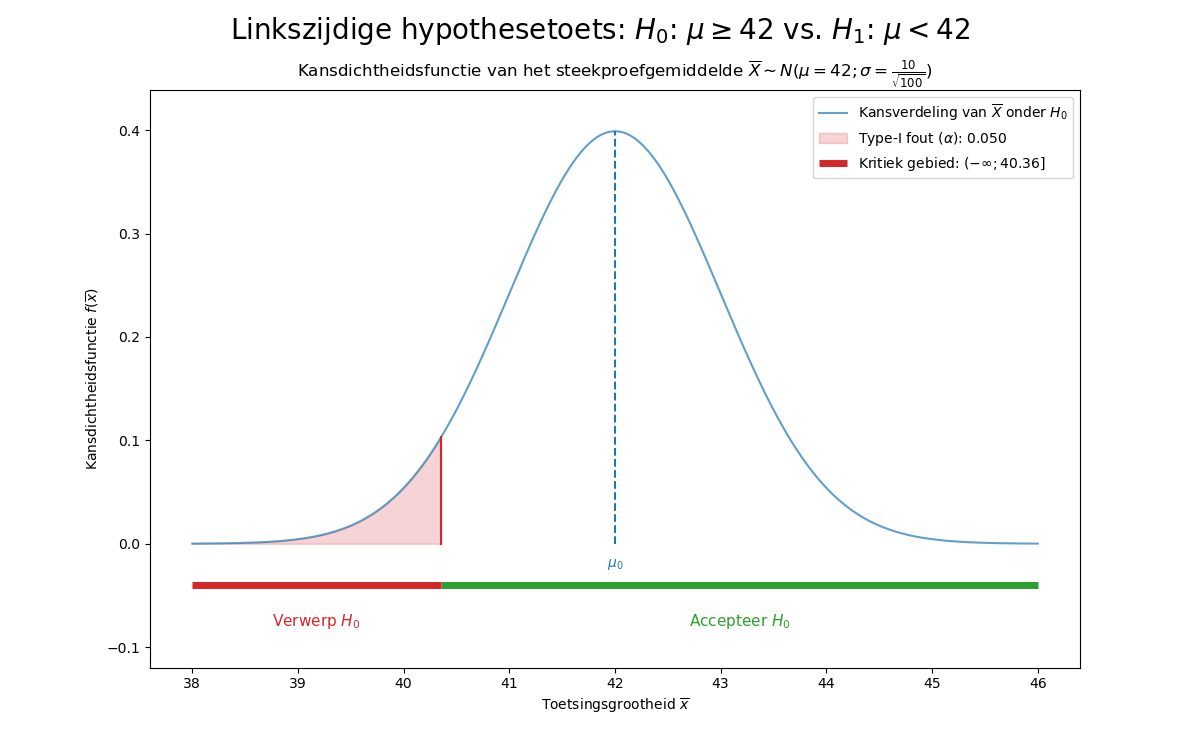
\includegraphics{opg_9.5.png}
        }
    \end{center}
}